\documentclass[UTF8]{ctexart}
\usepackage{graphicx}
\usepackage{amsmath}
\usepackage{enumerate}
\usepackage{cite}

\title{\heiti 《非定常空气动力学与分离流》 \\ 大作业}
\author{SX1501021 仓宇}
\date{\today}

\bibliographystyle{plain}

\begin{document}
\maketitle
\setcounter{page}{0}
\thispagestyle{empty}

\clearpage

\tableofcontents

\clearpage

\section{实验内容及要求}
\begin{enumerate}[(1)]
\item 采用三角剖分方法或非线性代数模型建模。
\item 样本数据为某飞机模型单自由度偏航运动风洞试验中测得的偏航力矩系数。数据文件名为ba1.dat$\sim$ba7.dat,运动规律为:
\[\psi_j=-24^\circ \cos(2\pi f)\]
$f$分别对应运动频率0.1Hz$\sim$0.7Hz,$\psi_j$对应数据文件中“psij”列。试验风速$v=25m/s$,模型展长0.75m。
\item 要求编写建模程序(语言不限),根据建模精度,调整系数个数,给出系数矩阵。
\item 根据建模结果,计算如下4项运动的偏航力矩迟滞环:
\begin{center} $\psi_j=-24^\circ \cos(2\pi f), f=0.35Hz$\end{center}
\begin{center} $\psi_j=-10^\circ-5^\circ \cos(2\pi f), f=0.2Hz$ \end{center}
\begin{center} $\psi_j=10^\circ-5^\circ \cos(2\pi f),f=0.2Hz$ \end{center}
\begin{center} $\psi_j=-5^\circ \cos(2\pi f), f=0.2Hz$ \end{center}
\item 给出计算曲线,如下图所示:
\begin{center}
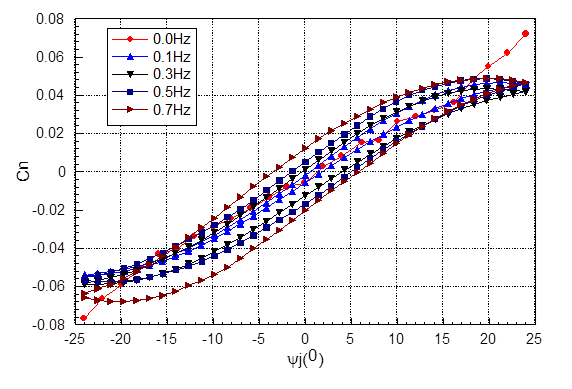
\includegraphics[width=10cm]{./src.png}
\end{center}
\end{enumerate}

\section{思路}
非线性代数模型的表达形式较简单,便于应用,但对于不同实验模型必须建立不同的数学模型表达式。基于数据库的阶跃函数模型虽然没有明确表达式,但是其计算精度较高,可以用于与其它模型结果进行比较\cite{shizhiwei1}。因此本实验采用基于数据库的三角剖分插值方法。\medskip \\
\indent 模型在单自由度运动时,其上的非定常气动力可视为一个二元函数,该二元函数的自变量是在该自由度上的位移和速率,速率的引入体现了了非定常项气动力的来源,具有一定的合理性。该自由度上的位移与速率构成了一个平面点集,三角剖分的思路就是找到待测点在这一平面点集中所处的三角形,然后得到待测点在这一小三角形上的面积坐标,最后按比例估算待测点的值。然而在一些特殊的情况下,待测点可以同时属于多个小三角形,因此如何划分给定的平面点集需要一定的考量。\medskip \\
\indent 直观地,我们可以发现若一个剖分产生了较多的较为狭长的小三角形,那么这个剖分会使得在狭长边附近的插值点的结果变化较快,插值点稍有变化将会导致结果的大幅度变化,因此是不稳定的。自然,我们要想办法尽量避免这些狭长的三角形,也就是避免三角剖分中含有过小的夹角。\medskip \\
\indent 设P为任一平面点集,根据计算几何中的知识可知P的任一角度最优的三角剖分必是P的一个Delaunay三角剖分,同时Delaunay三角剖分使得最小角达到最大,这样可使得插值的结果尽可能合乎实际。因此本实验使采用Delaunay三角剖分方法,将偏航方向的位移与速率映射为一平面点集,然后在其上进行插值。\medskip \\
\indent 程序流程如下:\\
\begin{center}
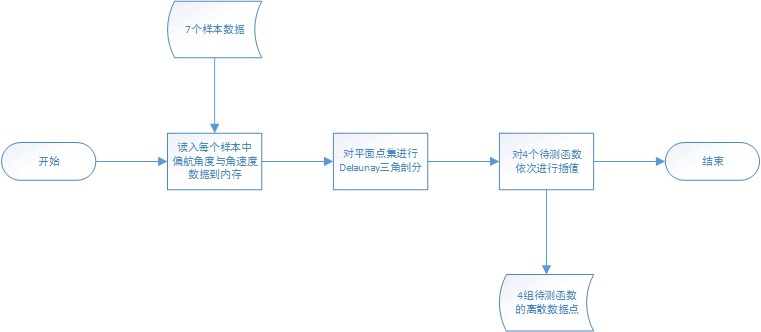
\includegraphics[width=9cm, height=5cm]{../tool/flowchart.png}
\end{center}

\section{编程实现}
Delaunay三角剖分是计算几何领域中的一个经典的案例,该算法有多种实现方式,常用的是基于随机增量方法的实现。CGAL(Computational Geometry Algorithms Library)是用C++语言实现的一个高效、可靠的计算几何算法库,被广泛应用于与计算几何紧密相关的领域。为了不纠缠于三角剖分算法实现的细节,本实验调用CGAL中与Delaunay三角剖分有关的接口,给定点集后由CGAL直接得到一个可靠的Delaunay三角剖分。\\
\indent 本实验中,二维点集的两个变量分别是$\psi_j$和$\dot{\psi_j}$,待测值是$C_n$。借助于CGAL与Qt,我们可以显示出由本实验的样本点所构成的二维Delaunay三角剖分,剖分图如下所示,横向表示$\psi_j$,纵向表示$\dot{\psi_j}$。\\
\begin{center}
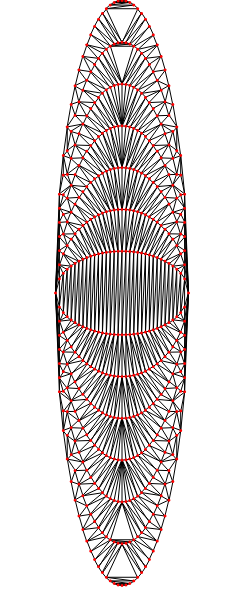
\includegraphics[width=6cm, height=8cm]{../results/raw_img.PNG}
\end{center}

\indent 得到样本点集的Delaunay三角剖分后就可以进行插值估算了。对给定的4个待测函数,为了使最后得到的曲线尽量平滑,每个待测函数取80个待测点,插值结果输出到results文件夹下。最后由Excel处理出对应的迟滞环。\\
\indent 由于CGAL使用了Boost和Qt中的功能,因此在搭建开发环境的时候需要先安装Qt并编译生成Boost链接库文件,本实验的操作平台是Window\ 7(64-bit) + Visual\ Studio\  2013(64-bit) + Boost-1.61.0 + CGAL-4.8,为了编译CGAL及关联项使用了Cmake-3.3.2,为了进行2D显示使用了Qt-5.6.0。由于牵涉到的软件较多,在配置开发环境的时候需要仔细而全面,否则会因为频繁的编译错误而浪费时间。也许在linux下开发环境的搭建会较为简单,但由于时间关系本次实验未做相关尝试。

\section{实验结果与分析}

\begin{enumerate}[a)]

\item $\psi_j=-24^\circ \cos(2\pi f), f=0.35Hz$ \\ 
\indent 由80个插值点得到的近似曲线如下:
\begin{center}
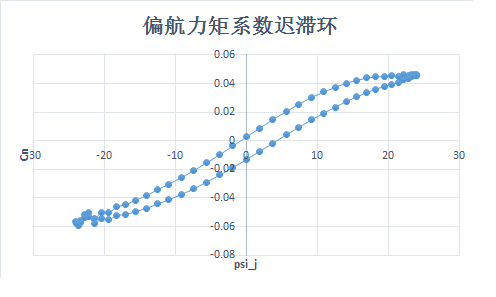
\includegraphics[width=10cm,height=5cm]{../results/case1.png}
\end{center}
\indent 由图可知在振幅大、频率较高时,非定常气动力的迟滞特性较为明显。

\item $\psi_j=-10^\circ-5^\circ \cos(2\pi f), f=0.2Hz$ \\ 
\indent 由80个插值点得到的近似曲线如下:
\begin{center}
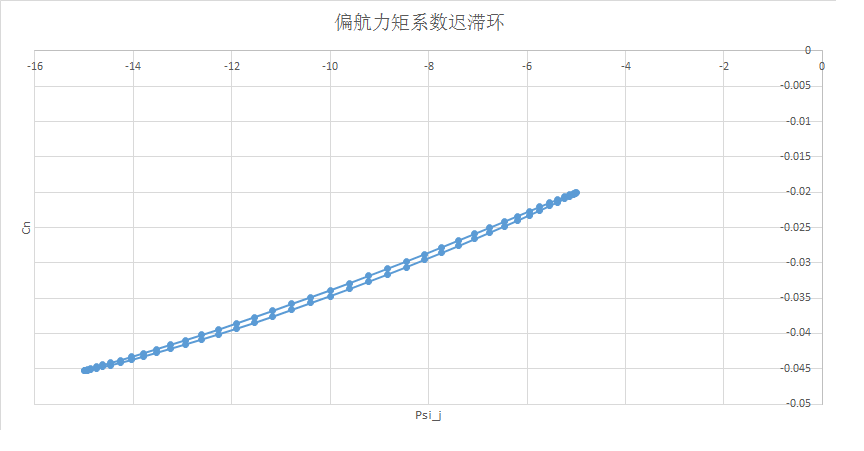
\includegraphics[width=10cm,height=5cm]{../results/case2.png}
\end{center}
\indent 由图可知在振幅较小、频率不高时,非定常气动力的迟滞特性不明显。

\item $\psi_j=10^\circ-5^\circ \cos(2\pi f),f=0.2Hz$ \\ 
\indent 由80个插值点得到的近似曲线如下:
\begin{center}
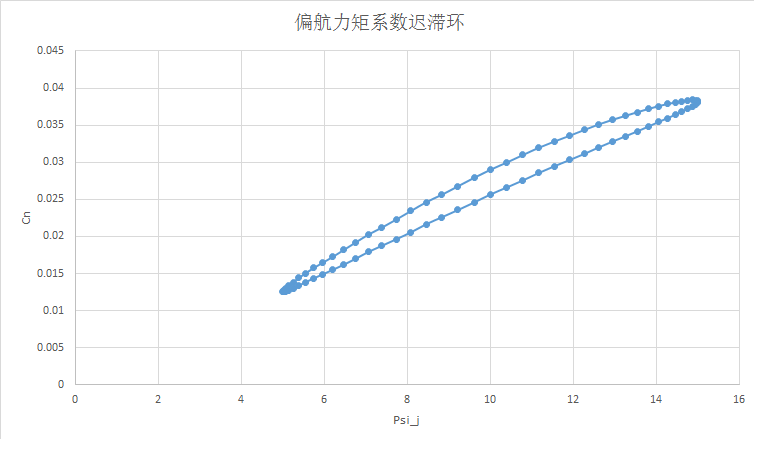
\includegraphics[width=8cm]{../results/case3.png}
\end{center}
\indent 相比于上例的负振幅,在振幅相同、频率相同时,运动方向的改变对非定常气动力的迟滞特性影响较大,但考虑到对称性,这一结果的可信度不高。

\item $\psi_j=-5^\circ \cos(2\pi f), f=0.2Hz$ \\ 
\indent 由80个插值点得到的近似曲线如下:
\begin{center}
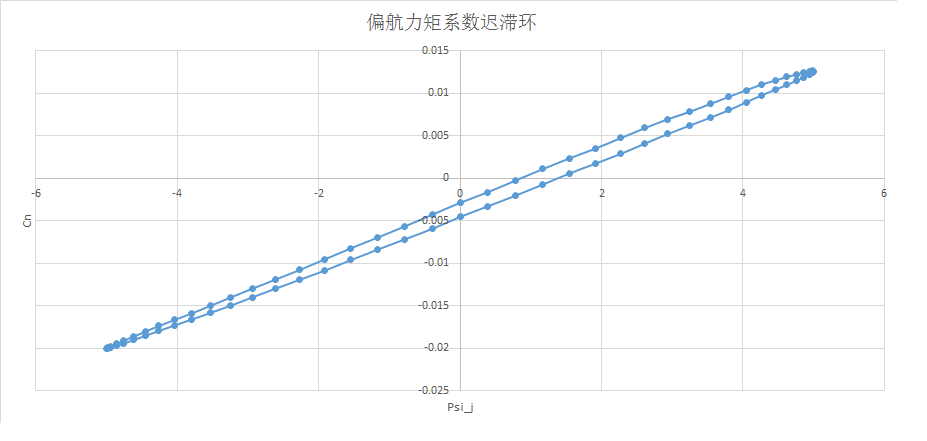
\includegraphics[width=8cm]{../results/case4.png}
\end{center}
\indent 由图可知在小振幅、低频率的情况下,非定常气动力的迟滞特性不太明显,$C_n$与$\psi_j$近似为线性关系

\end{enumerate}

\section{结论}
本次实验采用Delaunay三角剖分的方法对样本数据进行建模,并对4种非定常运动进行插值计算。计算结果表明:
\begin{enumerate}[(1)]
\item 在大振幅、高频率的情况下非定常气动力的迟滞特性很明显。
\item 随着振幅和频率的降低,非定常气动力的迟滞特性减弱,但在同一自由度上正反两个方向上的运动特性却有较大差别。
\item 随着振幅和频率的进一步降低,非定常气动力的迟滞特性进一步减弱,在整个运动范围内近似表现为线性特征。
\end{enumerate}

\clearpage

\addcontentsline{toc}{section}{参考文献}
\bibliography{unsteady}

\end{document}





































